\begin{Example}[mental3]{Mental impairment and parents' SES}
Cumulative logit models may be fit using \PROC{CATMOD} with the
\pname{RESPONSE CLOGIT;} statement.
The model is specified in the same way as for adjacent category
logits, but now the \verb|_RESPONSE_| keyword refers to
differences among the cumulative response probabilities.
As before,
an independent variable is treated as a quantitative variable,
when it is declared in a \stmt{DIRECT}{CATMOD}.

The following statements fit
the same models as in \exref{ex:mental4}: first Models 0--3
in which SES has no effect on mental health (Model 0), then SES with
a nominal effect (Model 1), a constant linear effect (Model 2)
and different linear effects for each cumulative logit (Model 3).
%% input: /users/faculty/friendly/sasuser/catdata/mental3.sas
%% last modified: 26-Nov-98 17:27
\begin{listing}
%include catdata(mental);

*-- Cumulative logit models;
proc catmod data=mental;
   weight count;
   population ses;
   response clogit / out=pred0;
   model mental = _response_ / noprofile noresponse title='Model 0: _R_';
  run;
   response clogit / out=pred1;
   model mental = _response_  ses / noprofile noresponse title='Model 1: _R_ SES';
  run;
   direct ses;
   response clogit / out=pred2;
   model mental = _response_  ses / noprofile noresponse title='Model 2:  _R_ S';
  run;
   direct ses;
   response clogit / out=pred3;
   model mental = _response_ | ses / noprofile noresponse title='Model 3:  _R_|S';
  run;
\end{listing}


For comparison, we also fit models with both linear and quadratic
effects on the cumulative logits,
first with equal slopes and curvature
for all response categories (Model 4), and second with separate slopes and
equal curvatures (Model 5).
%% input: /users/faculty/friendly/sasuser/catdata/mental3.sas
%% last modified: 29-Nov-98 11:55
\begin{listing}
data mental;
   set mental;
   ses2 = ses**2;

proc catmod data=mental;
   weight count;
   population ses;
   direct ses ses2;
   response clogit / out=pred4;
   model mental = _response_ ses ses2 / noprofile noiter title='Model 4: _R_ S S^2';
  run;
   response clogit / out=pred5;
   model mental = _response_|ses ses2 / noprofile noiter title='Model 5: _R_|S S^2';
  run;
\end{listing}


The model fit statistics for these models are shown in \tabref{tab:mentab3}.
The values are quite similar to those for the adjacent category logits
(\tabref{tab:mentab2}).
\begin{table}[htb]
 \caption{Cumulative logit models for Mental Health data}\label{tab:mentab3}
 \begin{center}
 \begin{tabular}{c l rrr r}
  \hline
  Model & Terms        & df & \chisq & $p$-value & AIC\\ 
  \hline
  0 & \verb\_R_\       & 15 & 45.92 & 0.0001 &  15.92\\ 
  1 & \verb\_R_| SES\  & 10 &  7.75 & 0.6536 & -12.25\\ 
  2 & \verb\_R_ S\     & 14 & 10.72 & 0.7080 & -17.28\\ 
  3 & \verb\_R_|S\     & 12 &  6.48 & 0.8897 & -17.52\\ 
  4 & \verb\_R_ S S^2\ & 13 &  8.36 & 0.8192 & -17.64\\ 
  5 & \verb\_R_|S S^2\ & 11 &  3.94 & 0.9716 & -18.06\\ 
  \hline
 \end{tabular}
 \end{center}
\end{table}


For any such model, the \macro{CATPLOT} displays the observed and fitted
cumulative logits using the \ODS\ specified on the
\stmt{RESPONSE}{CATMOD}.
The statements below produce the graphs of the logits for Model 0,
and Model 1,
shown in \figref{fig:mental3a}.
Similar statements, using the \ODS s \pname{PRED2} and \pname{PRED4},
give the graphs for Model 2 and Model 4 in \figref{fig:mental3b}.
%% input: /users/faculty/friendly/sasuser/catdata/mental3.sas
%% last modified: 02-Dec-98 15:47
\begin{listing}
axis1 label=(a=90);
axis2 offset=(3,6);
proc format;
   value cum 1='>1'  2='>2'  3='>3';
title 'Model 0: Mental = _R_';
%catplot(data=pred0, x=ses, y=_obs_, class=_number_, clfmt=cum.,
   type=FUNCTION, ylab=Cumulative Logit);
title 'Model 1: Mental = _R_ SES';
%catplot(data=pred1, x=ses, y=_obs_, class=_number_, clfmt=cum.,
   type=FUNCTION, ylab=Cumulative Logit);
\end{listing}


%% two subfig side-by-side
\begin{figure}[htb]
 \begin{minipage}[t]{.49\linewidth}
  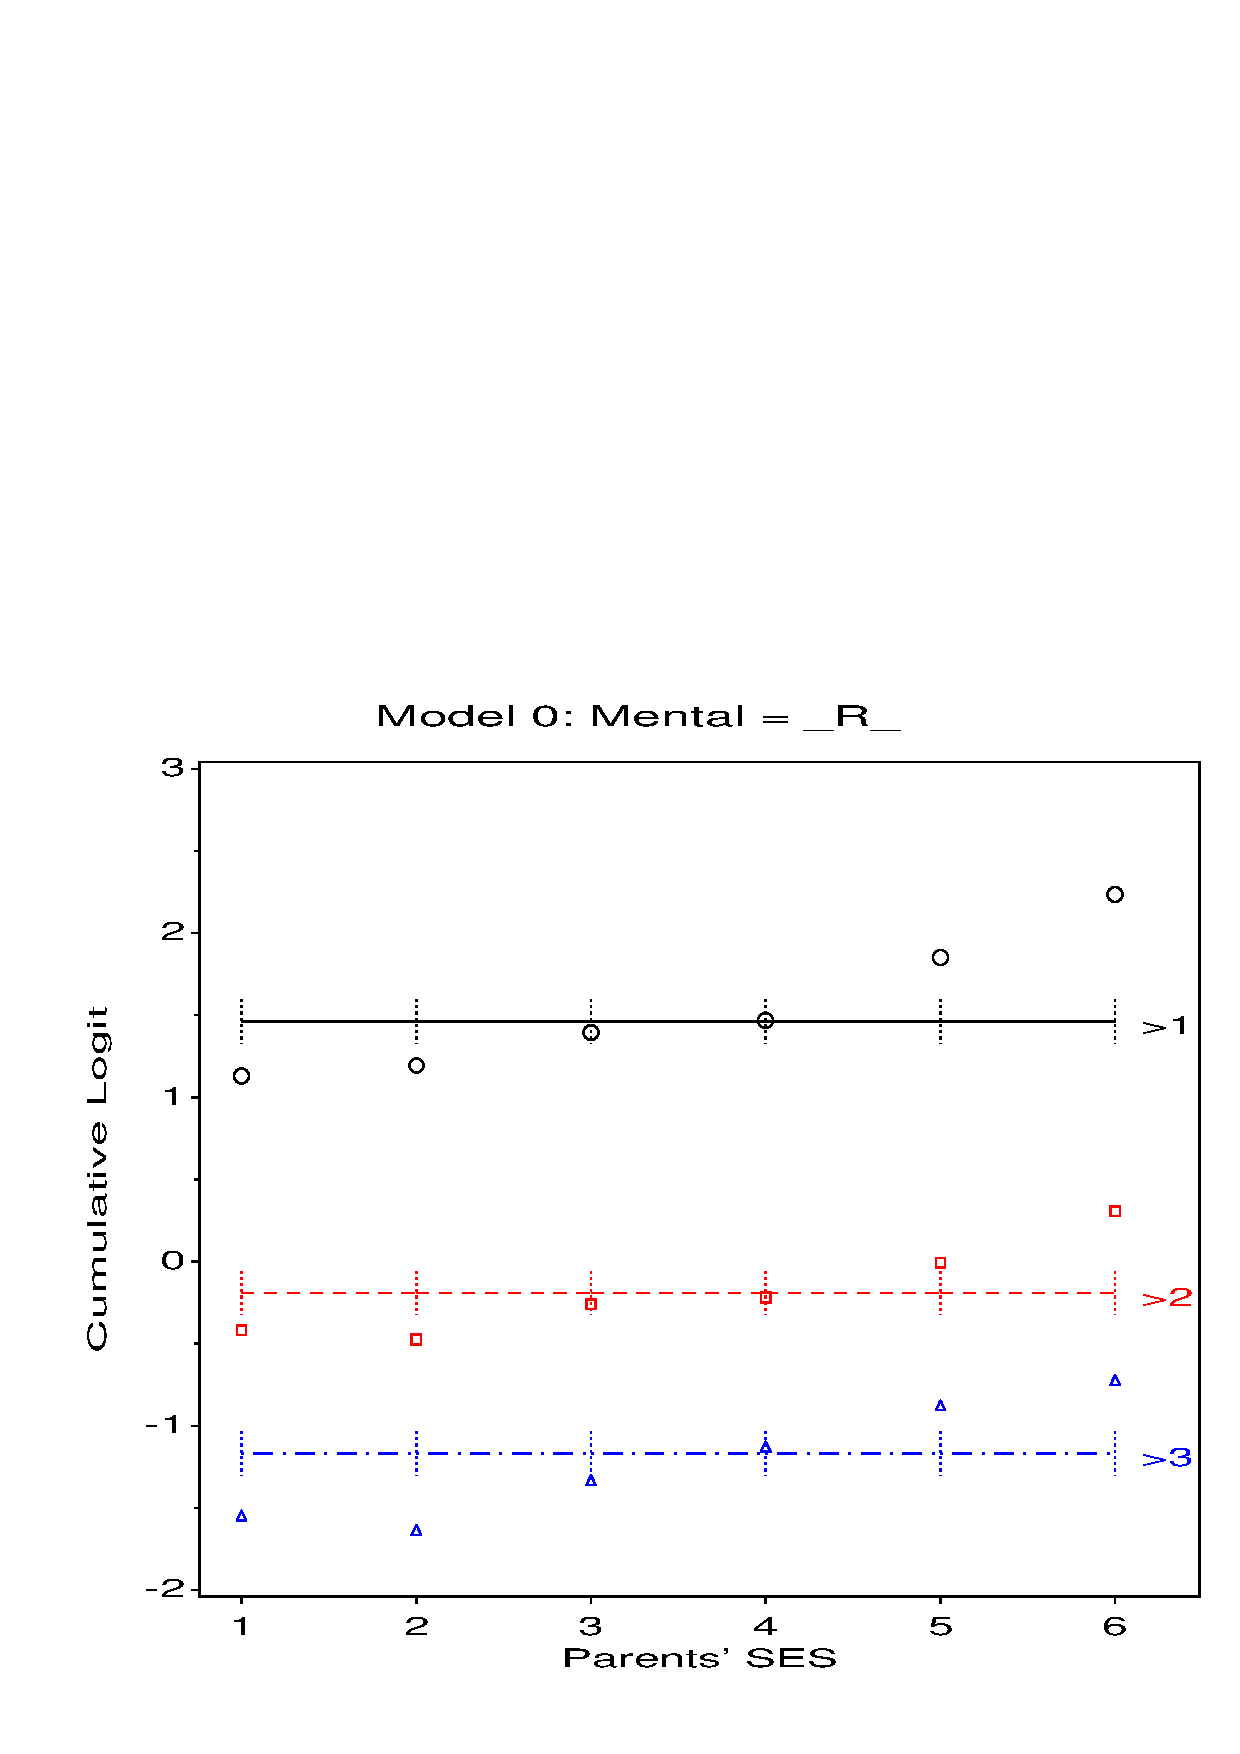
\includegraphics[width=1\linewidth]{mental31}
 \end{minipage}%
 \hfill
 \begin{minipage}[t]{.49\linewidth}
  \includegraphics[width=1\linewidth]{mental32}
 \end{minipage}
 \caption{Cumulative logit models for Mental Health data, Model 0 and Model 1}\label{fig:mental3a}
\end{figure}

%% two subfig side-by-side
\begin{figure}[htb]
 \begin{minipage}[t]{.49\linewidth}
  \includegraphics[width=1\linewidth]{mental33}
 \end{minipage}%
 \hfill
 \begin{minipage}[t]{.49\linewidth}
  \includegraphics[width=1\linewidth]{mental35}
 \end{minipage}
 \caption{Cumulative logit models for Mental Health data: Model 2 and Model 4}\label{fig:mental3b}
\end{figure}
\end{Example}